\chapter{Đọc thêm 3: Nội suy Spline}
\label{ch:M1L3-reading}

\section{Phương pháp Nội suy Spline}

\subsection{Tại sao chúng ta cần Nội suy Spline?}

\subsubsection{Mục tiêu Học tập}
Sau khi hoàn thành thành công bài học này, bạn sẽ có khả năng:
1) giải thích tại sao nội suy bậc cao là một ý tưởng tồi,
2) cách nội suy spline có thể tránh được những cạm bẫy của nội suy bậc cao.

\subsubsection{Giới thiệu}
Nội suy đa thức liên quan đến việc tìm một đa thức bậc $n$ hoặc nhỏ hơn đi qua $n+1$ điểm. Một số phương pháp để thu được đa thức như vậy bao gồm phương pháp trực tiếp (còn gọi là phương pháp đa thức Vandermonde), phương pháp đa thức sai phân chia Newton, và phương pháp nội suy Lagrange.

Vậy phương pháp spline có phải là một phương pháp khác để thu được đa thức bậc $n$ này không? KHÔNG!
Thực tế, khi $n$ trở nên lớn, trong nhiều trường hợp, ta có thể gặp phải hành vi dao động trong đa thức nội suy. Hiện tượng này đã được Runge minh họa khi ông nội suy dữ liệu dựa trên một hàm đơn giản
\begin{equation}
y=\frac{1}{1+25x^{2}}
\end{equation}
trên một khoảng $[-1,1]$.

Ví dụ, lấy sáu điểm cách đều nhau trong $[-1,1]$ và tìm $y$ tại các điểm này từ Phương trình (5.5.1.1). Các giá trị này được cho trong Bảng 5.5.1.1.

\begin{table}[h]
\centering
\begin{tabular}{|c|c|}
\hline
$x$ & $y=\frac{1}{1+25x^{2}}$ \\
\hline
-1.0 & 0.038461 \\
-0.6 & 0.1 \\
-0.2 & 0.5 \\
0.2 & 0.5 \\
0.6 & 0.1 \\
1.0 & 0.038461 \\
\hline
\end{tabular}
\caption{Sáu điểm cách đều nhau trong $[-1,1]$.}
\end{table}

Bây giờ đi qua sáu điểm dữ liệu này, ta có thể xây dựng một đa thức nội suy bậc năm.
\begin{equation}
f_{5}(x)=1.2019x^{4}-1.7308x^{2}+0.56731 \quad -1\le x\le1
\end{equation}
Khi vẽ đồ thị đa thức bậc năm (Phương trình (5.5.1.2)) và hàm ban đầu (Phương trình (5.5.1.1)), như thấy ở Hình 5.5.1.1, bạn có thể thấy rằng chúng không khớp nhau tốt. Đa thức có đi qua sáu cặp dữ liệu của Bảng 5.5.1.1, nhưng nó thậm chí không đến gần hàm ban đầu tại nhiều điểm khác. Chỉ cần nhìn vào $x=0.85$, giá trị của hàm ban đầu là 0.052459, nhưng đa thức bậc năm cho bạn giá trị là -0.055762. Đó là một sai số thực tương đối khổng lồ lên tới 206.30\%.

\begin{figure}[htbp]
    \centering
    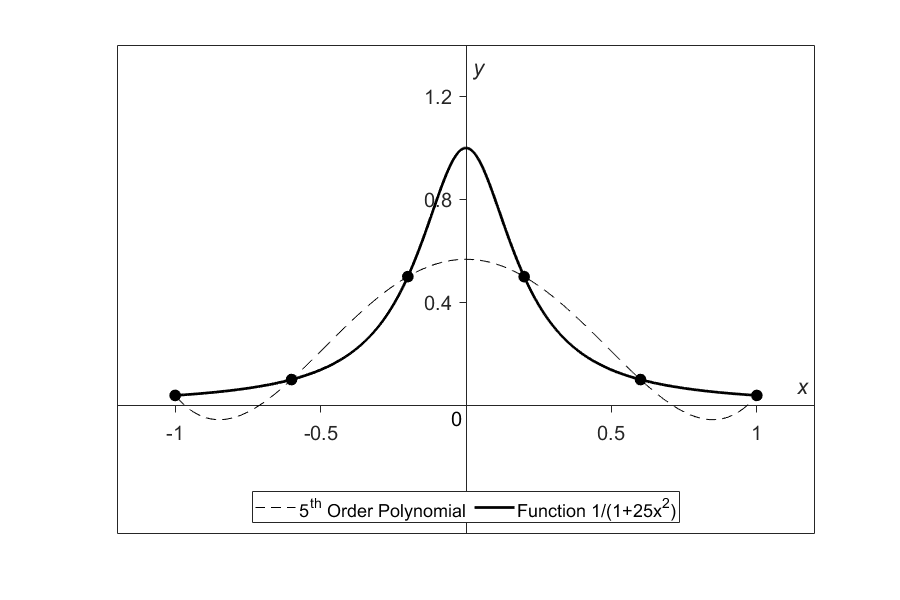
\includegraphics[width=0.8\textwidth]{gfx/m1l3_spline_runge_5th_order.png}
    \caption{Nội suy đa thức bậc năm với sáu điểm cách đều nhau.}
    \label{fig:spline_runge_5th_order}
\end{figure}

Người ta có thể nghĩ rằng việc chọn nhiều điểm hơn trong khoảng $[-1,1]$ sẽ cho chúng ta sự khớp tốt hơn giữa hàm ban đầu và hàm nội suy, nhưng nó thậm chí còn phân kỳ nhiều hơn (Hình 5.5.1.2). Ở đây, 20 điểm cách đều nhau đã được chọn trong khoảng $[-1,1]$ để vẽ một đa thức nội suy bậc 19. Tuy nhiên, nó đã làm tốt hơn việc xấp xỉ dữ liệu nhưng ngoại trừ gần các đầu mút nơi xấp xỉ tồi tệ hơn trước. Tại điểm đã chọn, $x=0.85$ giá trị của hàm ban đầu là 0.052459, trong khi ta nhận được -0.62944 từ đa thức bậc 19. Điều đó gây ra một sai số thực tương đối lớn tới 1299.9\%.

Trên thực tế, Runge phát hiện ra rằng khi bậc của đa thức tiến tới vô cùng, đa thức càng phân kỳ hơn trong khoảng $-1<x<-0.726$ và $0.726<x<1$.

\begin{figure}[htbp]
    \centering
    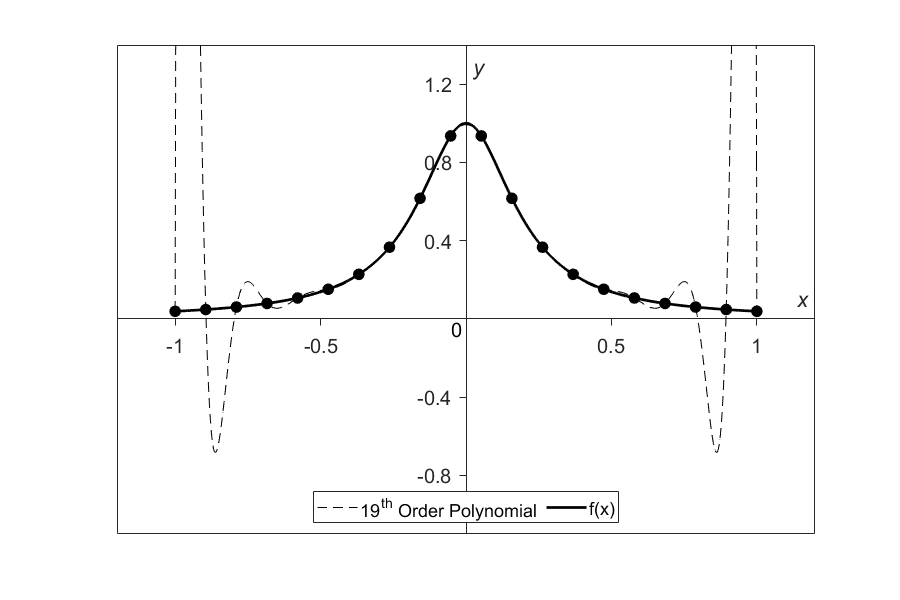
\includegraphics[width=0.8\textwidth]{gfx/m1l3_spline_runge_19th_order.png}
    \caption{Nội suy đa thức bậc mười chín với hai mươi điểm cách đều nhau.}
    \label{fig:spline_runge_19th_order}
\end{figure}

Vậy, giải pháp cho việc sử dụng thông tin từ nhiều điểm dữ liệu hơn, mà vẫn giữ cho hàm số tương đối trung thực với hành vi của dữ liệu là gì? Câu trả lời nằm ở nội suy spline và sẽ được thảo luận trong các bài học sau. Các loại nội suy spline phổ biến nhất được sử dụng là tuyến tính, bậc hai và bậc ba.

\subsection{Nội suy Spline Tuyến tính}

\subsubsection{Mục tiêu Học tập}
Sau khi hoàn thành thành công bài học này, bạn sẽ có khả năng:
1) phát triển hàm nội suy spline tuyến tính cho các điểm dữ liệu cho trước,
2) ước tính các điểm dữ liệu chưa biết từ hàm nội suy spline tuyến tính.

\subsubsection{Nội suy Spline Tuyến tính}
Cho $(x_{0},y_{0}),(x_{1},y_{1}),......,(x_{n-1},y_{n-1}),(x_{n},y_{n})$ , hãy tìm spline tuyến tính nội suy (Hình 5.5.2.1) cho dữ liệu. Quá trình này đơn giản chỉ liên quan đến việc vẽ các đường thẳng giữa các điểm liên tiếp.

\begin{figure}[htbp]
    \centering
    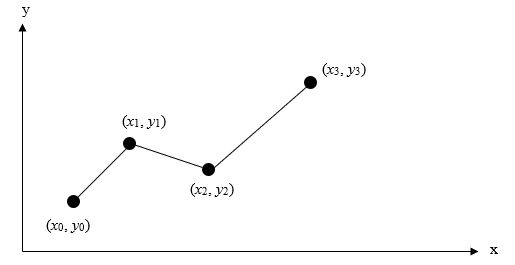
\includegraphics[width=0.8\textwidth]{gfx/m1l3_spline_piecewise_linear_points.png}
    \caption{Spline tuyến tính.}
    \label{fig:spline_piecewise_linear_points}
\end{figure}

Giả sử rằng dữ liệu trên được cho theo thứ tự tăng dần, spline tuyến tính nội suy, còn được gọi là spline bậc 1, $f(x)$ được cho bởi:
\begin{align}
f(x) &= f(x_0) + \frac{f(x_1)-f(x_0)}{x_1-x_0}(x-x_0), \quad x_0 \le x \le x_1 \\
&= f(x_1) + \frac{f(x_2)-f(x_1)}{x_2-x_1}(x-x_1), \quad x_1 \le x \le x_2 \\
&\vdots \nonumber \\
&= f(x_{n-1}) + \frac{f(x_n)-f(x_{n-1})}{x_n-x_{n-1}}(x-x_{n-1}), \quad x_{n-1} \le x \le x_n \label{eq:5.5.2.1}
\end{align}

Lưu ý rằng $y_{i}=f(x_{i})$ trong biểu thức trên và các số hạng của
\begin{equation}
\frac{f(x_{i})-f(x_{i-1})}{x_{i}-x_{i-1}}
\end{equation}
chỉ đơn giản là các độ dốc giữa $x_{i-1}$ và $x_i$.

\subsubsection{Ví dụ}
Vận tốc hướng lên của một tên lửa được cho như một hàm của thời gian trong Bảng 5.5.2.1 (Hình 5.5.2.2).

\begin{table}[h]
\centering
\begin{tabular}{|c|c|}
\hline
$t(s)$ & $v(t)$ $(m/s)$ \\
\hline
0 & 0 \\
10 & 227.04 \\
15 & 362.78 \\
20 & 517.35 \\
22.5 & 602.97 \\
30 & 901.67 \\
\hline
\end{tabular}
\caption{Vận tốc như một hàm của thời gian.}
\end{table}

Hãy xác định giá trị của vận tốc tại $t=16$ giây bằng cách sử dụng một spline tuyến tính nội suy.

\begin{figure}[htbp]
    \centering
    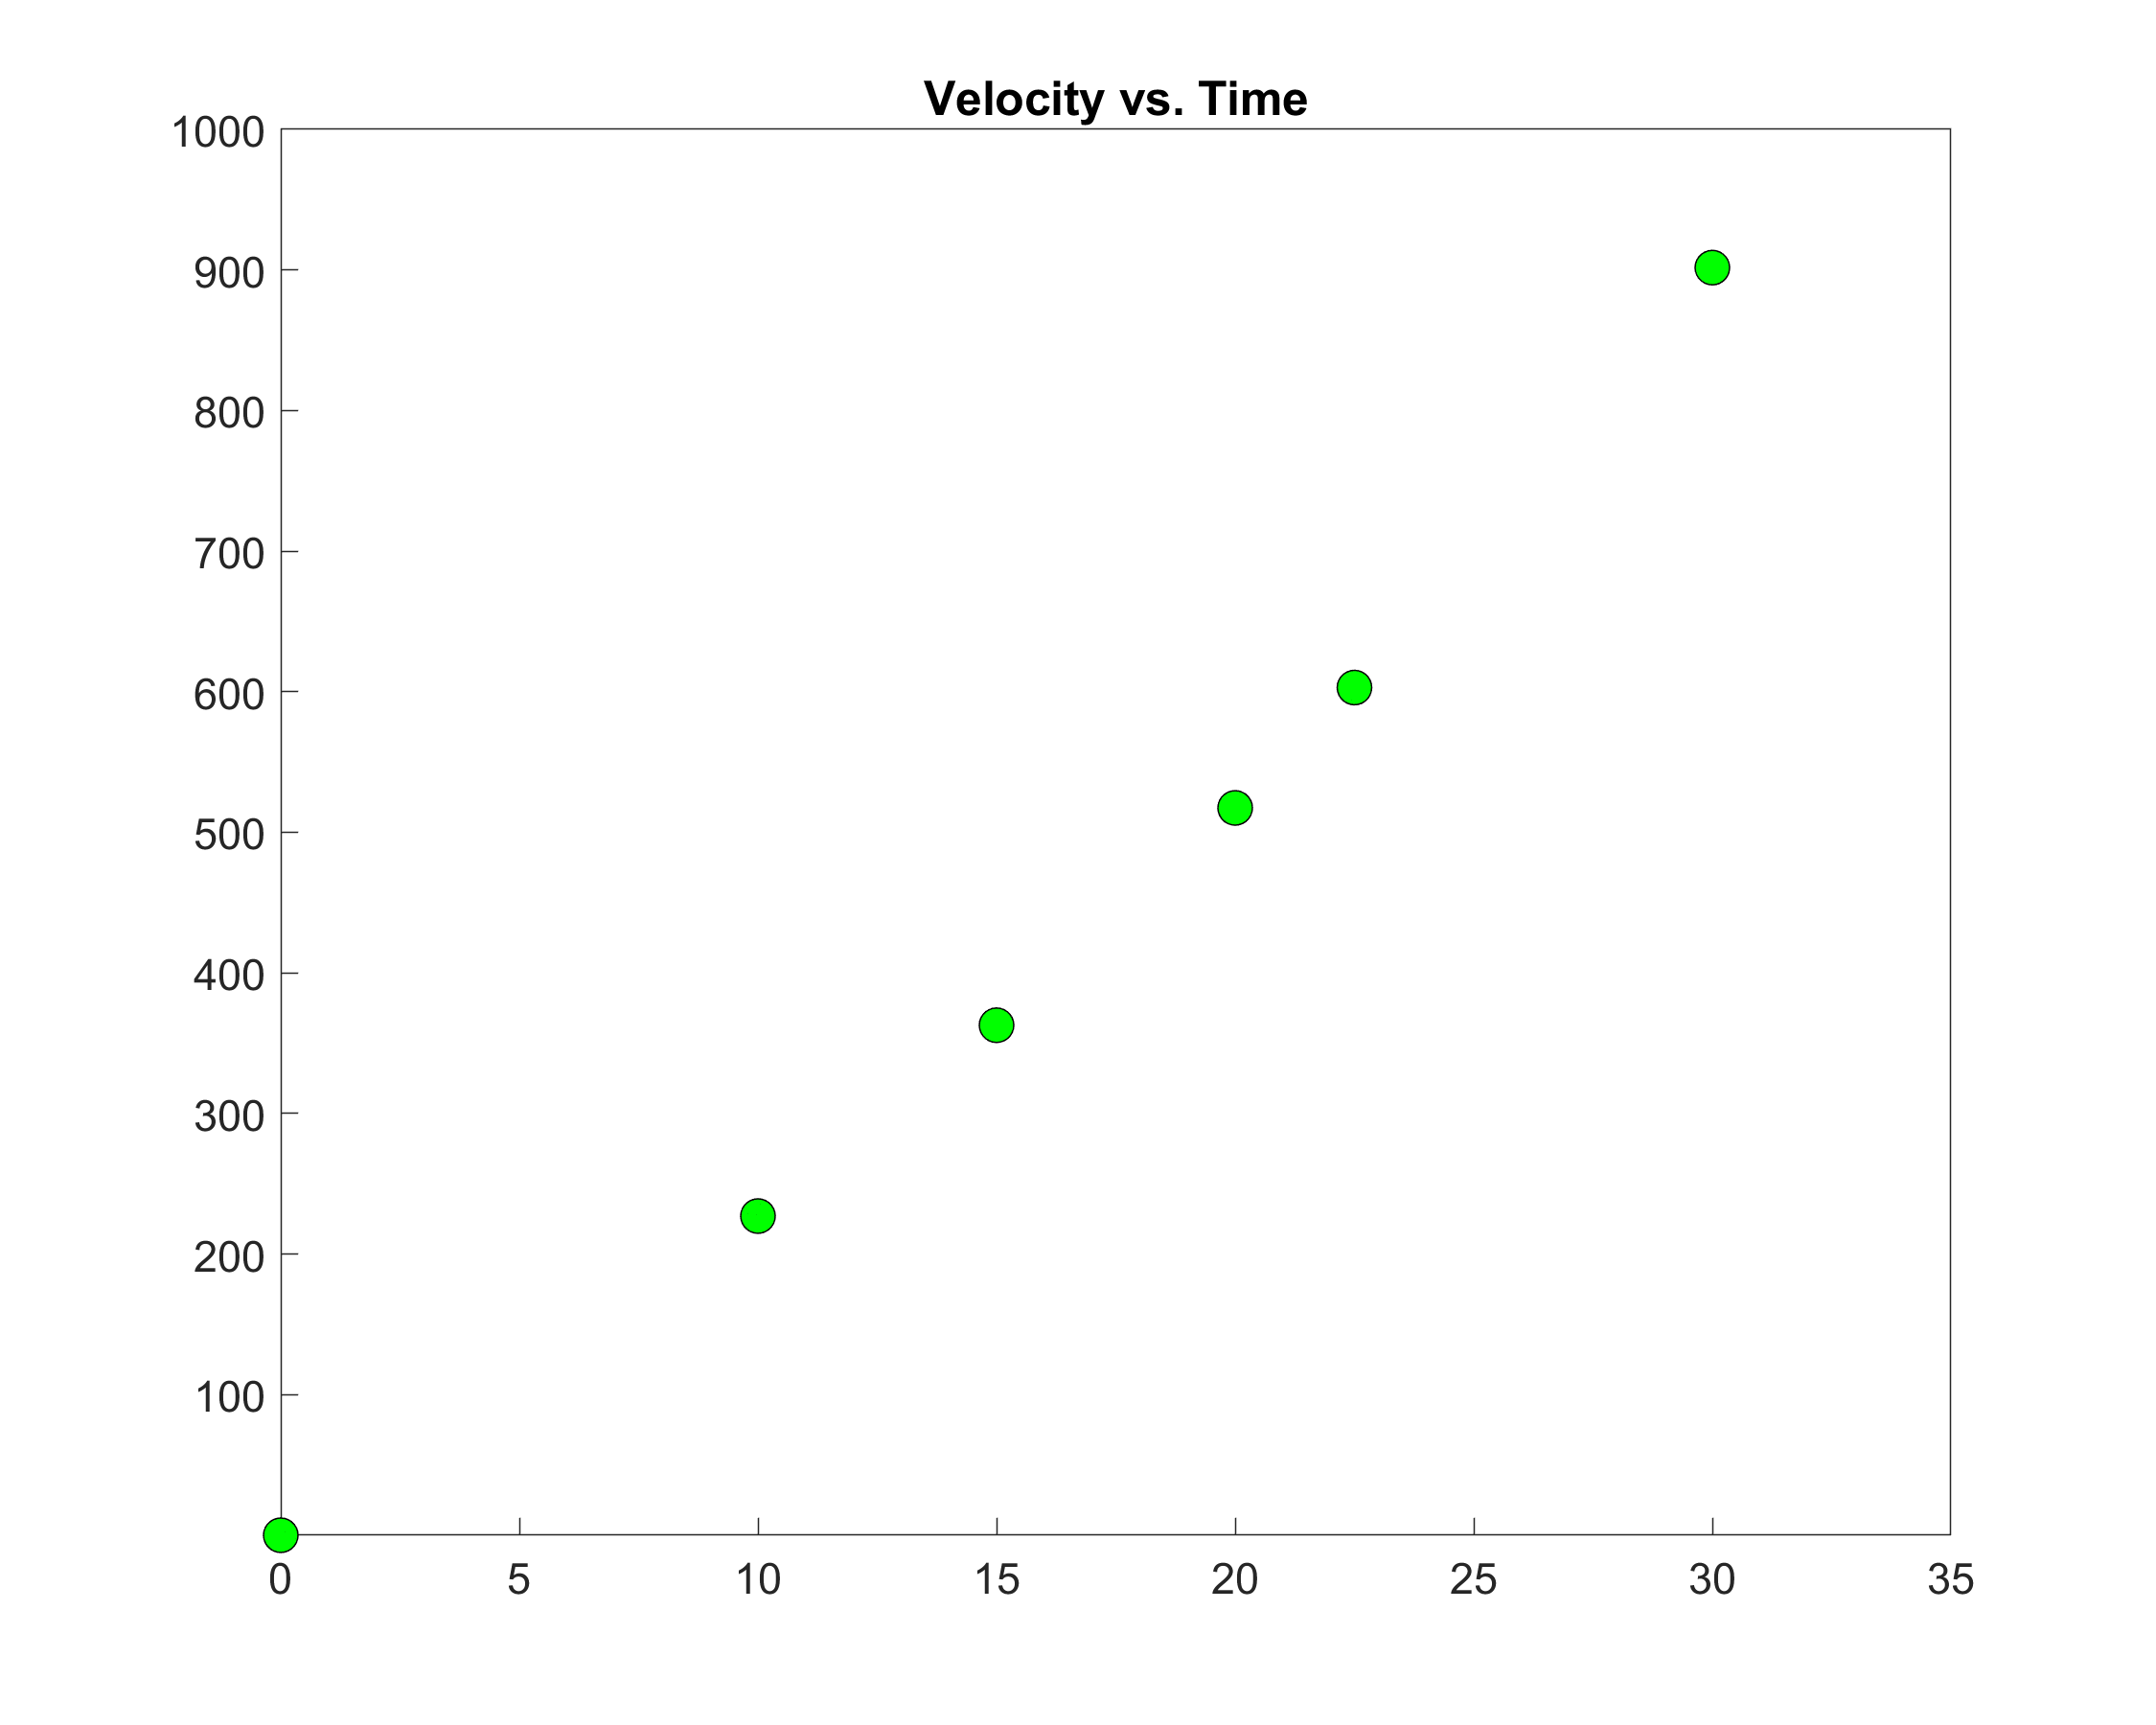
\includegraphics[width=0.8\textwidth]{gfx/m1l3_spline_velocity_vs_time.png}
    \caption{Đồ thị dữ liệu vận tốc theo thời gian cho ví dụ về tên lửa.}
    \label{fig:spline_velocity_vs_time}
\end{figure}

\textbf{Giải}

Vì chúng ta muốn tính vận tốc tại $t=16$ và sử dụng nội suy spline tuyến tính, chúng ta cần chọn hai điểm dữ liệu gần $t=16$ nhất đồng thời bao quanh $t=16$ để đánh giá nó. Hai điểm đó là $t_{0}=15$ và $t_{1}=20$

Khi đó
$t_{0}=15$, $v(t_{0})=362.78$ \\
$t_{1}=20$, $v(t_{1})=517.35$

mang lại
\begin{align*}
v(t) &= v(t_0) + \frac{v(t_1)-v(t_0)}{t_1-t_0}(t-t_0) \\
&= 362.78 + \frac{517.35-362.78}{20-15}(t-15) \\
&= 362.78 + 30.913(t-15) \quad 15 \le t \le 20
\end{align*}

Tại $t=16$,
\begin{align*}
v(16) &= 362.78 + 30.913(16-15) \\
&= 393.7~m/s
\end{align*}

Nội suy spline tuyến tính không khác gì nội suy đa thức tuyến tính. Nội suy spline tuyến tính vẫn chỉ sử dụng dữ liệu từ hai điểm dữ liệu liên tiếp, và dữ liệu từ các điểm khác hoàn toàn không được sử dụng. Ngoài ra, tại các điểm bên trong của dữ liệu, độ dốc của spline thay đổi đột ngột, điều này ngụ ý rằng đạo hàm bậc nhất "một cách giả tạo" không liên tục tại các điểm này. Vậy chúng ta vượt qua hai nhược điểm này như thế nào? Chúng ta có thể làm như vậy bằng cách sử dụng nội suy spline bậc hai hoặc bậc ba. Chúng ta sẽ thảo luận về các loại nội suy spline này trong các bài học sắp tới.

\subsection{Nội suy Spline Bậc hai}

\subsubsection{Mục tiêu Học tập}
Sau khi hoàn thành thành công bài học này, bạn sẽ có khả năng:
1) suy ra spline bậc hai nội suy cho dữ liệu rời rạc.

\subsubsection{Spline Bậc hai Nội suy}
Nội suy spline bậc hai là một phương pháp để khớp đường cong với dữ liệu. Đối với nội suy spline bậc hai, các hàm bậc hai từng phần xấp xỉ dữ liệu giữa hai điểm dữ liệu liên tiếp (Hình 5.5.3.1). Cho $(x_{0},y_{0}),(x_{1},y_{1}),.............,(x_{n-1},y_{n-1}),(x_{n},y_{n})$, khớp một spline bậc hai nội suy qua dữ liệu. Các hàm bậc hai của spline được cho bởi
\begin{align}
f(x) &= a_1x^2 + b_1x + c_1, \quad x_0 \le x \le x_1 \\
&= a_2x^2 + b_2x + c_2, \quad x_1 \le x \le x_2 \\
&\vdots \nonumber \\
&= a_nx^2 + b_nx + c_n, \quad x_{n-1} \le x \le x_n
\end{align}

Vậy làm thế nào để tìm các hệ số của các hàm bậc hai này? Có $3n$ hệ số như vậy:
$a_i, i=1,2,......,n$ \\
$b_i, i=1,2,.......,n$ \\
$c_i, i=1,2,.....,n$

Để tìm $3n$ ẩn số, người ta cần thiết lập $3n$ phương trình và sau đó giải đồng thời chúng. Các $3n$ phương trình này được tìm như sau.

\begin{figure}[htbp]
    \centering
    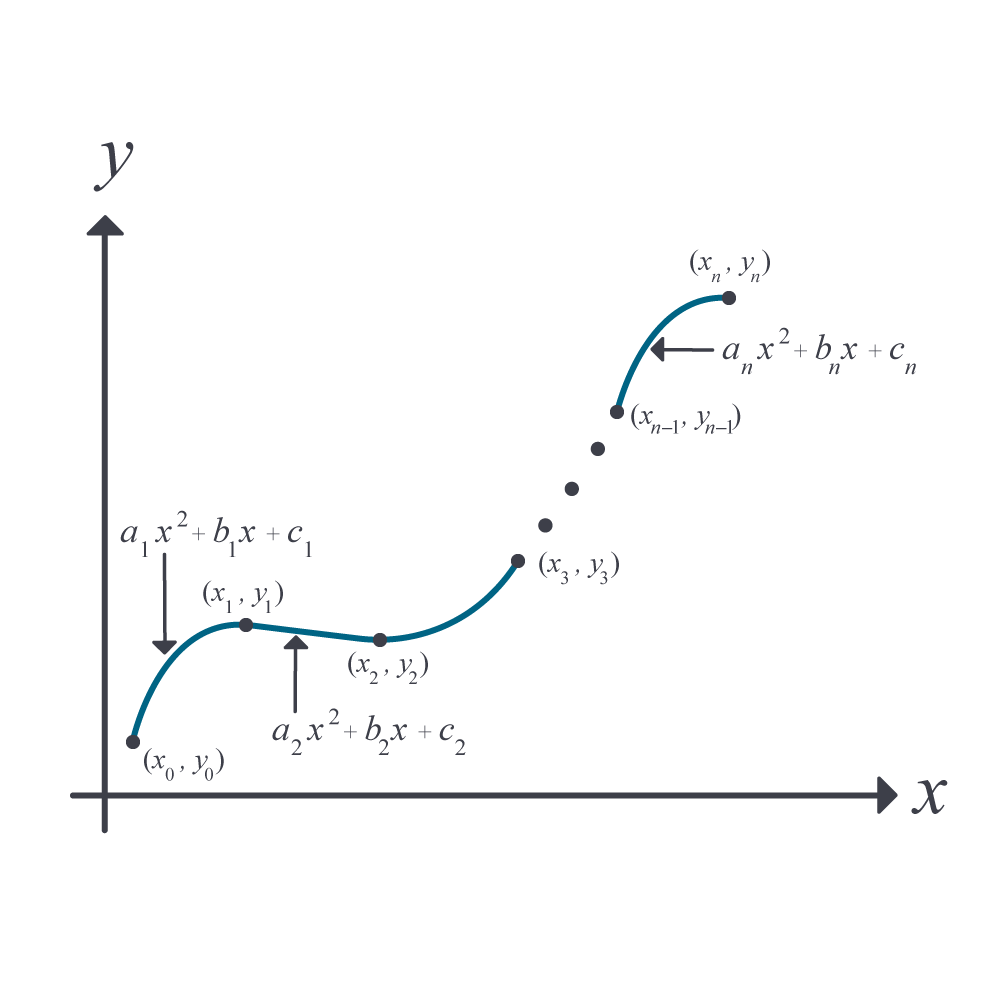
\includegraphics[width=0.8\textwidth]{gfx/m1l3_spline_quadratic_segments.png}
    \caption{Nội suy spline bậc hai}
    \label{fig:spline_quadratic_segments}
\end{figure}

1. Mỗi hàm bậc hai đi qua hai điểm dữ liệu liên tiếp:
\begin{align}
a_1{x_0}^2 + b_1x_0 + c_1 &= f(x_0) \nonumber \\
a_1{x_1}^2 + b_1x_1 + c_1 &= f(x_1) \nonumber \\
&\vdots \nonumber \\
a_i{x_{i-1}}^2 + b_ix_{i-1} + c_i &= f(x_{i-1}) \\
a_i{x_i}^2 + b_ix_i + c_i &= f(x_i) \nonumber \\
&\vdots \nonumber \\
a_n{x_{n-1}}^2 + b_nx_{n-1} + c_n &= f(x_{n-1}) \nonumber \\
a_n{x_n}^2 + b_nx_n + c_n &= f(x_n) \nonumber
\end{align}
Điều kiện này cho $2n$ phương trình vì có $n$ hàm bậc hai đi qua hai điểm dữ liệu liên tiếp.

2. Đạo hàm bậc nhất của hai hàm bậc hai liên tiếp là liên tục tại các điểm bên trong chung. Ví dụ, đạo hàm của hàm bậc hai thứ nhất $a_{1}x^{2}+b_{1}x+c_{1}$ là $2a_{1}x+b_{1}$. Đạo hàm của hàm bậc hai thứ hai $a_{2}x^{2}+b_{2}x+c_{2}$ là $2a_{2}x+b_{2}$, và hai giá trị này bằng nhau tại điểm bên trong chung $x=x_{1}$, mang lại:
$$2a_{1}x_{1}+b_{1}=2a_{2}x_{1}+b_{2}$$
$$2a_{1}x_{1}+b_{1}-2a_{2}x_{1}-b_{2}=0$$

Tương tự, tại các điểm bên trong khác $x_{2},...,x_{n-1}$
\begin{align}
2a_2x_2 + b_2 - 2a_3x_2 - b_3 &= 0 \nonumber \\
&\vdots \nonumber \\
2a_ix_i + b_i - 2a_{i+1}x_i - b_{i+1} &= 0 \\
&\vdots \nonumber \\
2a_{n-1}x_{n-1} + b_{n-1} - 2a_nx_{n-1} - b_n &= 0 \nonumber
\end{align}
Vì có $(n-1)$ điểm bên trong, chúng ta có $(n-1)$ phương trình như vậy.

3. Cho đến nay, tổng số phương trình thu được là $(2n)+(n-1)=(3n-1)$ phương trình. Vậy chúng ta vẫn cần thêm một phương trình nữa. Chúng ta có thể giả định hàm bậc hai đầu tiên là tuyến tính, tức là $a_{1}=0$. Một số người giả định hàm bậc hai cuối cùng là tuyến tính, tức là $a_{n}=0$.
Những người khác dựa trên cơ sở khoảng nào nhỏ hơn, $[x_{0},x_{1}]$ hoặc $[x_{n-1},x_{n}]$. Nếu $|x_{1}-x_{0}|\le|x_{n}-x_{n-1}|$, thì người ta sẽ chọn $a_{1}=0$; nếu không, chọn $a_{n}=0$.

Điều này cho chúng ta $3n$ phương trình tuyến tính đồng thời và $3n$ ẩn. Chúng có thể được giải bằng một số kỹ thuật dùng để giải hệ phương trình tuyến tính đồng thời tổng quát.

\subsection{Ứng dụng của Nội suy Spline Bậc hai}

\subsubsection{Mục tiêu Học tập}
Sau khi hoàn thành thành công bài học này, bạn sẽ có khả năng:
1) thực hiện nội suy spline bậc hai trên dữ liệu rời rạc,
2) đạo hàm một spline bậc hai nội suy khi cần thiết,
3) tích phân một spline bậc hai nội suy khi cần thiết.

\subsubsection{Các Ứng dụng}
Trong bài học trước, bạn đã tìm hiểu lý thuyết về phương pháp nội suy spline bậc hai. Trong bài học này, chúng tôi áp dụng lý thuyết để nội suy dữ liệu rời rạc cho trước thành một spline bậc hai nội suy.

\textbf{Ví dụ} \\
Vận tốc hướng lên của một tên lửa được cho như một hàm của thời gian là \\
Bảng 5.5.4.1. Vận tốc như một hàm của thời gian.

\begin{table}[h]
\centering
\begin{tabular}{|c|c|}
\hline
$t(s)$ & $v(t)$ $(m/s)$ \\
\hline
0 & 0 \\
10 & 227.04 \\
15 & 362.78 \\
20 & 517.35 \\
22.5 & 602.97 \\
30 & 901.67 \\
\hline
\end{tabular}
\end{table}

a) Xác định giá trị của vận tốc tại $t=16$ giây sử dụng nội suy spline bậc hai. \\
b) Sử dụng spline bậc hai nội suy, tìm quãng đường tên lửa đi được từ $t=11$ s đến $t=16$ s. \\
c) Sử dụng spline bậc hai nội suy, tìm gia tốc của tên lửa tại $t=16$ s.

\textbf{Giải} \\
a) Vì có sáu điểm dữ liệu, năm hàm bậc hai sẽ đi qua chúng.
\begin{align}
v(t) &= a_1t^2 + b_1t + c_1, \quad 0 \le t \le 10 \nonumber \\
&= a_2t^2 + b_2t + c_2, \quad 10 \le t \le 15 \nonumber \\
&= a_3t^2 + b_3t + c_3, \quad 15 \le t \le 20 \\
&= a_4t^2 + b_4t + c_4, \quad 20 \le t \le 22.5 \nonumber \\
&= a_5t^2 + b_5t + c_5, \quad 22.5 \le t \le 30 \nonumber
\end{align}

Các phương trình được tìm như sau. \\
1. Mỗi hàm bậc hai đi qua hai điểm dữ liệu liên tiếp. \\
Hàm bậc hai $a_{1}t^{2}+b_{1}t+c_{1}$ đi qua $t=0$ và $t=10$. \\
$a_{1}(0)^{2}+b_{1}(0)+c_{1}=0$ (5.5.4.E1.1) \\
$a_{1}(10)^{2}+b_{1}(10)+c_{1}=227.04$ (5.5.4.E1.2) \\
Hàm bậc hai $a_{2}t^{2}+b_{2}t+c_{2}$ đi qua $t=10$ và $t=15$. \\
$a_{2}(10)^{2}+b_{2}(10)+c_{2}=227.04$ (5.5.4.E1.3) \\
$a_{2}(15)^{2}+b_{2}(15)+c_{2}=362.78$ (5.5.4.E1.4) \\
Hàm bậc hai $a_{3}t^{2}+b_{3}t+c_{3}$ đi qua $t=15$ và $t=20$. \\
$a_{3}(15)^{2}+b_{3}(15)+c_{3}=362.78$ (5.5.4.E1.5) \\
$a_{3}(20)^{2}+b_{3}(20)+c_{3}=517.35$ (5.5.4.E1.6) \\
Hàm bậc hai $a_{4}t^{2}+b_{4}t+c_{4}$ đi qua $t=20$ và $t=22.5$. \\
$a_{4}(20)^{2}+b_{4}(20)+c_{4}=517.35$ (5.5.4.E1.7) \\
$a_{4}(22.5)^{2}+b_{4}(22.5)+c_{4}=602.97$ (5.5.4.E1.8) \\
Hàm bậc hai $a_{5}t^{2}+b_{5}t+c_{5}$ đi qua $t=22.5$ và $t=30$. \\
$a_{5}(22.5)^{2}+b_{5}(22.5)+c_{5}=602.97$ (5.5.4.E1.9) \\
$a_{5}(30)^{2}+b_{5}(30)+c_{5}=901.67$ (5.5.4.E1.10) 

2. Các hàm bậc hai có các đạo hàm liên tục tại các điểm dữ liệu bên trong chung. \\
Tại $t=10$: $2a_{1}(10)+b_{1}-2a_{2}(10)-b_{2}=0$ (5.5.4.E1.11) \\
Tại $t=15$: $2a_{2}(15)+b_{2}-2a_{3}(15)-b_{3}=0$ (5.5.4.E1.12) \\
Tại $t=20$: $2a_{3}(20)+b_{3}-2a_{4}(20)-b_{4}=0$ (5.5.4.E1.13) \\
Tại $t=22.5$: $2a_{4}(22.5)+b_{4}-2a_{5}(22.5)-b_{5}=0$ (5.5.4.E1.14)

3. Giả sử hàm bậc hai cuối cùng $a_{5}t^{2}+b_{5}t+c_{5}$ là tuyến tính (tại sao chúng ta chọn spline cuối cùng là tuyến tính thay vì cái đầu tiên?), \\
$a_{5}=0$ (5.5.4.E1.15)

Kết hợp các Phương trình từ (5.5.4.E1.1) đến (5.5.4.E1.15) dưới dạng ma trận ta được
\begin{align*}
\left[
\begin{array}{*{15}{c}}
0 & 0 & 1 & 0 & 0 & 0 & 0 & 0 & 0 & 0 & 0 & 0 & 0 & 0 & 0 \\
100 & 10 & 1 & 0 & 0 & 0 & 0 & 0 & 0 & 0 & 0 & 0 & 0 & 0 & 0 \\
0 & 0 & 0 & 100 & 10 & 1 & 0 & 0 & 0 & 0 & 0 & 0 & 0 & 0 & 0 \\
0 & 0 & 0 & 225 & 15 & 1 & 0 & 0 & 0 & 0 & 0 & 0 & 0 & 0 & 0 \\
0 & 0 & 0 & 0 & 0 & 0 & 225 & 15 & 1 & 0 & 0 & 0 & 0 & 0 & 0 \\
0 & 0 & 0 & 0 & 0 & 0 & 400 & 20 & 1 & 0 & 0 & 0 & 0 & 0 & 0 \\
0 & 0 & 0 & 0 & 0 & 0 & 0 & 0 & 0 & 400 & 20 & 1 & 0 & 0 & 0 \\
0 & 0 & 0 & 0 & 0 & 0 & 0 & 0 & 0 & 506.25 & 22.5 & 1 & 0 & 0 & 0 \\
0 & 0 & 0 & 0 & 0 & 0 & 0 & 0 & 0 & 0 & 0 & 0 & 506.25 & 22.5 & 1 \\
0 & 0 & 0 & 0 & 0 & 0 & 0 & 0 & 0 & 0 & 0 & 0 & 900 & 30 & 1 \\
20 & 1 & 0 & -20 & -1 & 0 & 0 & 0 & 0 & 0 & 0 & 0 & 0 & 0 & 0 \\
0 & 0 & 0 & 30 & 1 & 0 & -30 & -1 & 0 & 0 & 0 & 0 & 0 & 0 & 0 \\
0 & 0 & 0 & 0 & 0 & 0 & 40 & 1 & 0 & -40 & -1 & 0 & 0 & 0 & 0 \\
0 & 0 & 0 & 0 & 0 & 0 & 0 & 0 & 0 & 45 & 1 & 0 & -45 & -1 & 0 \\
0 & 0 & 0 & 0 & 0 & 0 & 0 & 0 & 0 & 0 & 0 & 0 & 1 & 0 & 0 
\end{array}
\right]
\begin{bmatrix}
a_1 \\ b_1 \\ c_1 \\ a_2 \\ b_2 \\ c_2 \\ a_3 \\ b_3 \\ c_3 \\ a_4 \\ b_4 \\ c_4 \\ a_5 \\ b_5 \\ c_5
\end{bmatrix}
=
\begin{bmatrix}
0 \\ 227.04 \\ 227.04 \\ 362.78 \\ 362.78 \\ 517.35 \\ 517.35 \\ 602.97 \\ 602.97 \\ 901.67 \\ 0 \\ 0 \\ 0 \\ 0 \\ 0
\end{bmatrix}
\end{align*}

Giải 15 phương trình tuyến tính đồng thời trên cho 15 ẩn số ta được
\begin{table}[h]
\centering
\begin{tabular}{|c|c|c|c|}
\hline
$i$ & $a_i$ & $b_i$ & $c_i$ \\
\hline
1 & -0.15667 & 24.271 & 0 \\
2 & 1.2021 & -2.9053 & 135.88 \\
3 & -0.44893 & 46.627 & -235.61 \\
4 & 2.2315 & -60.589 & 836.55 \\
5 & 0 & 39.827 & -293.13 \\
\hline
\end{tabular}
\end{table}

Do đó, spline bậc hai nội suy được cho bởi
\begin{align}
v(t) &= -0.15667t^2 + 24.271t, \quad 0 \le t \le 10 \nonumber \\
&= 1.2021t^2 - 2.9053t + 135.88, \quad 10 \le t \le 15 \nonumber \\
&= -0.44893t^2 + 46.627t - 235.61, \quad 15 \le t \le 20 \\
&= 2.2315t^2 - 60.589t + 836.55, \quad 20 \le t \le 22.5 \nonumber \\
&= 39.827t - 293.13, \quad 22.5 \le t \le 30 \nonumber
\end{align}

Tại $t=16~s$
\begin{align}
v(16) &= -0.44893(16)^2 + 46.627(16) - 235.61 \nonumber \\
&= 395.50~m/s
\end{align}

b) Quãng đường tên lửa đi được từ 11 s đến 16 s giây có thể được tính như sau
\begin{equation}
s(16)-s(11)=\int_{11}^{16}v(t)dt
\end{equation}

Nhưng vì có vài hàm bậc hai có hiệu lực qua các cận tích phân, chúng ta cần chia tích phân một cách tương ứng. Sử dụng Phương trình (5.5.4.E1.16).
\begin{align}
v(t) &= 1.2021t^2 - 2.9053t + 135.88, \quad 10 \le t \le 15 \nonumber \\
&= -0.44893t^2 + 46.627t - 235.61, \quad 15 \le t \le 20
\end{align}

Sau đó
\begin{align}
s(16)-s(11) &= \int_{11}^{16}v(t)dt \nonumber \\
&= \int_{11}^{15}v(t)dt+\int_{15}^{16}v(t)dt
\end{align}

Thay thế các hàm bậc hai thích hợp mang lại
\begin{align}
s(16)-s(11) &= \int_{11}^{15} (1.2021t^2 - 2.9053t + 135.88) dt \nonumber \\
&\quad + \int_{15}^{16} (-0.44893t^2 + 46.627t - 235.61) dt \nonumber \\
&= \left[1.2021\frac{t^3}{3} - 2.9053\frac{t^2}{2} + 135.88t\right]_{11}^{15} \\
&\quad + \left[-0.44893\frac{t^3}{3} + 46.627\frac{t^2}{2} - 235.61t\right]_{15}^{16} \nonumber \\
&= 1211.49 + 379.22 \nonumber \\
&= 1590.7~m \nonumber
\end{align}

c) Gia tốc tại $t=16~s$ là bao nhiêu?
\begin{equation}
a(16)=\frac{dv}{dt}\bigg|_{t=16}
\end{equation}

Ở đây chúng ta sử dụng hàm bậc hai thứ ba từ Phương trình (5.5.4.E1.15),
$$ -0.44893t^{2}+46.627t-235.61, \quad 15\le t\le20 $$
vì $t=16$ nằm trong miền của $15\le t\le20$.

Vậy
\begin{align}
a(t) &= \frac{d}{dt}v(t) \nonumber \\
&= \frac{d}{dt}(-0.44893t^2 + 46.627t - 235.61) \nonumber \\
&= -0.89786t + 46.627, \quad 15 \le t \le 20
\end{align}

\begin{align}
a(16) &= -0.89786(16) + 46.627 \nonumber \\
&= 32.261~m/s^2
\end{align}


\subsection{Phác thảo Nội suy Spline Bậc ba}

\subsubsection{Mục tiêu Học tập}
Sau khi hoàn thành thành công bài học này, bạn sẽ có khả năng:
1) phác thảo phép suy luận của nội suy spline bậc ba.

\subsubsection{Giới thiệu}
Giống như nội suy spline bậc hai, nội suy spline bậc ba là một phương pháp để khớp đường cong với dữ liệu. Nội suy spline bậc ba là bậc spline phổ biến nhất được sử dụng.

\subsubsection{Spline Bậc ba Nội suy}
Cho $n+1$ điểm dữ liệu, $(x_{0},y_{0}),$ $(x_{1},y_{1}),...,(x_{n},y_{n})$ hãy khớp một spline bậc ba nội suy qua dữ liệu. Đối với nội suy spline bậc ba, các đa thức bậc ba từng phần xấp xỉ dữ liệu giữa hai điểm liên tiếp. Spline bậc ba nội suy được cho bởi các đa thức bậc ba như
\begin{align}
f(x) &= a_1x^3 + b_1x^2 + c_1x + d_1, \quad x_0 \le x \le x_1 \nonumber \\
&= a_2x^3 + b_2x^2 + c_2x + d_2, \quad x_1 \le x \le x_2 \\
&\vdots \nonumber \\
&= a_nx^3 + b_nx^2 + c_nx + d_n, \quad x_{n-1} \le x \le x_n \nonumber
\end{align}

Vậy, làm thế nào để tìm các hệ số của những đa thức bậc ba này? Có $4n$ hệ số như vậy được đưa ra dưới đây.
\begin{align}
a_i, \quad & i=1,2,...,n \nonumber \\
b_i, \quad & \nonumber \\
c_i, \quad & \nonumber \\
d_i, \quad & i=1,2,...,n
\end{align}

Để tìm $4n$ ẩn số, chúng ta cần thiết lập $4n$ phương trình tuyến tính đồng thời. Khái quát việc thiết lập các phương trình này như sau.
Chúng ta có $n+1$ điểm dữ liệu. Trong số $n+1$ điểm này, hai là các điểm dữ liệu bên ngoài (đầu mút), trong khi có $(n+1)-2=n-1$ điểm dữ liệu bên trong.

1. Mỗi hàm bậc ba phải đi qua hai điểm liên tiếp. Vì chúng ta có $n$ spline, chúng ta sẽ nhận được $2n$ phương trình.
2. Đạo hàm bậc nhất của hai hàm bậc ba liên tiếp là liên tục tại điểm dữ liệu bên trong chung. Vì chúng ta có $(n-1)$ điểm bên trong, chúng ta sẽ nhận được $2(n-1)$ phương trình.
3. Đạo hàm bậc hai của hai hàm bậc ba liên tiếp là liên tục tại điểm dữ liệu bên trong chung. Vì chúng ta có $(n-1)$ điểm bên trong, chúng ta sẽ nhận được $2(n-1)$ phương trình.

Cho đến nay, chúng ta đã phác thảo rằng có thể thiết lập
\begin{equation}
(2n)+(n-1)+(n-1) = 4n-2
\end{equation}
phương trình. Chúng ta cần hai phương trình nữa, và một số loại điều kiện có thể được sử dụng để lấy chúng. Một vài điều kiện phổ biến được sử dụng như sau.
1. Giả sử rằng các spline bậc ba đầu tiên và cuối cùng là các hàm bậc hai $a_{1}=0$ và $a_{n}=0$ để nhận hai phương trình bổ sung. Giả định này được gọi là điều kiện biên bậc hai.
2. Giả sử đạo hàm bậc hai của spline bậc ba đầu tiên và cuối cùng là bằng không $(6a_{1}x_{0}+2b_{1}=0$ và $6a_{n}x_{n}+2b_{n}=0)$ tại các điểm bên ngoài tương ứng để nhận hai phương trình bổ sung. Giả định này được gọi là điều kiện biên tự nhiên.

\subsection{Bài kiểm tra Trắc nghiệm}

(1). $n$ điểm dữ liệu sau đây, $(x_{1},y_{1})$, $(x_{2},y_{2}),........(x_{n},y_{n})$, được cho. Để tiến hành nội suy spline bậc hai, dữ liệu x cần được
(A) cách đều nhau
(B) đặt theo thứ tự tăng dần hoặc giảm dần của các giá trị x
(C) số nguyên
(D) số dương

(2). Trong nội suy spline bậc ba,
(A) các đạo hàm bậc nhất của hàm bậc ba là liên tục tại các điểm dữ liệu bên trong
(B) các đạo hàm bậc hai của hàm bậc ba là liên tục tại các điểm dữ liệu bên trong
(C) các đạo hàm bậc nhất và bậc hai của hàm bậc ba là liên tục tại các điểm dữ liệu bên trong
(D) các đạo hàm bậc ba của hàm bậc ba là liên tục tại các điểm dữ liệu bên trong

(3). Dữ liệu y theo x chưa hoàn chỉnh sau đây được cho.
\begin{table}[h]
\centering
\begin{tabular}{|c|c|c|c|c|c|c|}
\hline
$x$ & 1 & 2 & 4 & 6 & 7 \\
\hline
$y$ & 5 & 11 & ???? & ???? & 32 \\
\hline
\end{tabular}
\end{table}

Dữ liệu được khớp bởi các spline bậc hai nội suy cho bởi
\begin{align}
f(x) &= ax-1, \quad 1 \le x \le 2 \nonumber \\
&= -2x^2+14x-9, \quad 2 \le x \le 4 \nonumber \\
&= bx^2+cx+d, \quad 4 \le x \le 6 \nonumber \\
&= 25x^2-303x+928, \quad 6 \le x \le 7
\end{align}
với a, b, c, và d là các hằng số. Giá trị của c gần nhất với
(A) -303.00
(B) -144.50
(C) 0.0000
(D) 14.000

(4). Dữ liệu y theo x chưa hoàn chỉnh sau đây được cho.
\begin{table}[h]
\centering
\begin{tabular}{|c|c|c|c|c|c|c|}
\hline
$x$ & 1 & 2 & 4 & 6 & 7 \\
\hline
$y$ & 5 & 11 & ???? & ???? & 32 \\
\hline
\end{tabular}
\end{table}

Dữ liệu được khớp bởi spline bậc hai nội suy cho bởi
\begin{align}
f(x) &= ax-1, \quad 1 \le x \le 2 \nonumber \\
&= -2x^2+14x-9, \quad 2 \le x \le 4 \nonumber \\
&= bx^2+cx+d, \quad 4 \le x \le 6 \nonumber \\
&= ex^2+fx+g, \quad 6 \le x \le 7
\end{align}
với a, b, c, d, e, f, và g là các hằng số. Giá trị của $\frac{df}{dx}$ tại $x=2.6$ gần nhất với
(A) -144.50
(B) -4.0000
(C) 3.6000
(D) 12.200

(5). Dữ liệu y theo x chưa hoàn chỉnh sau đây được cho.
\begin{table}[h]
\centering
\begin{tabular}{|c|c|c|c|c|c|c|}
\hline
$x$ & 1 & 2 & 4 & 6 & 7 \\
\hline
$y$ & 5 & 11 & ???? & ???? & 32 \\
\hline
\end{tabular}
\end{table}

Dữ liệu được khớp bởi spline bậc hai nội suy cho bởi
\begin{align}
f(x) &= ax-1, \quad 1 \le x \le 2, \nonumber \\
&= -2x^2+14x-9, \quad 2 \le x \le 4 \nonumber \\
&= bx^2+cx+d, \quad 4 \le x \le 6 \nonumber \\
&= 25x^2-303x+928, \quad 6 \le x \le 7
\end{align}
với a, b, c, và d là các hằng số. Giá trị ước tính của $\int_{1.5}^{3.5}f(x)dx$ là bao nhiêu?
(A) 23.500
(B) 25.667
(C) 25.750
(D) 28.000

(6). Một robot cần đi theo một con đường lần lượt đi qua sáu điểm như hình vẽ. Để tìm đường đi ngắn nhất mà cũng nhẵn, bạn sẽ đề xuất phương án nào sau đây?

\begin{figure}[htbp]
    \centering
    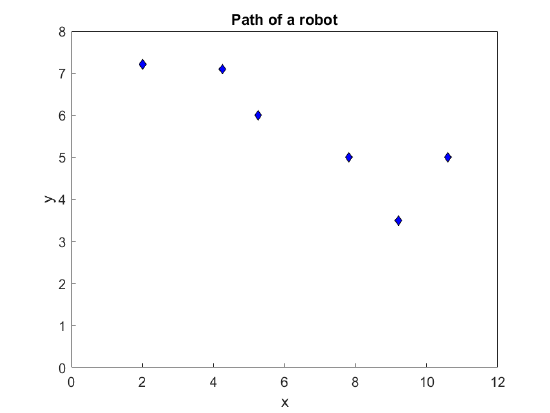
\includegraphics[width=0.8\textwidth]{gfx/m1l3_spline_path_of_robot.png}
    \caption{Đường đi của một con robot}
    \label{fig:spline_path_of_robot}
\end{figure}

(A) Cho một đa thức bậc năm đi qua dữ liệu
(B) Cho spline tuyến tính nội suy đi qua dữ liệu
(C) Cho spline bậc hai nội suy đi qua dữ liệu
(D) Hồi quy dữ liệu thành một đa thức bậc hai

\subsection{Bài tập}

(1). Dữ liệu y theo x sau đây được cho.
\begin{table}[h]
\centering
\begin{tabular}{|c|c|c|c|}
\hline
$x$ & 2 & 3 & 6 \\
\hline
$y$ & 4.75 & 5.25 & 45 \\
\hline
\end{tabular}
\end{table}

a) Thiết lập các phương trình để giải tìm spline bậc hai nội suy đi qua dữ liệu.
b) Sử dụng một chương trình như MATLAB để giải các phương trình và sau đó viết ra spline bậc hai nội suy.
c) Ước tính giá trị của $y(3.6)$.

\textbf{Trả lời} \\
a)
\begin{align*}
\begin{bmatrix}
4 & 2 & 1 & 0 & 0 & 0 \\
9 & 3 & 1 & 0 & 0 & 0 \\
0 & 0 & 0 & 9 & 3 & 1 \\
0 & 0 & 0 & 36 & 6 & 1 \\
6 & 1 & 0 & -6 & -1 & 0 \\
1 & 0 & 0 & 0 & 0 & 0
\end{bmatrix}
\begin{bmatrix}
a_1 \\ b_1 \\ c_1 \\ a_2 \\ b_2 \\ c_2
\end{bmatrix}
=
\begin{bmatrix}
4.75 \\ 5.25 \\ 5.25 \\ 45 \\ 0 \\ 0
\end{bmatrix}
\end{align*}

b)
\begin{table}[h]
\centering
\begin{tabular}{|c|c|c|c|}
\hline
$i$ & $a_i$ & $b_i$ & $c_i$ \\
\hline
1 & 0 & 0.5 & 3.75 \\
2 & 4.25 & -25 & 42 \\
\hline
\end{tabular}
\end{table}

c) 7.08

(2). Dữ liệu y theo x sau đây được cho.
\begin{table}[h]
\centering
\begin{tabular}{|c|c|c|c|c|c|}
\hline
$x$ & 1 & 2 & 3 & 5 & 6 \\
\hline
$y$ & 4.75 & 4 & 5.25 & 15 & 45 \\
\hline
\end{tabular}
\end{table}

Dữ liệu được khớp bởi spline bậc hai nội suy cho bởi
\begin{align}
f(x) &= -0.75x+5.5, \quad 1 \le x \le 2 \nonumber \\
&= 2x^2-8.75x+13.5, \quad 2 \le x \le 3 \nonumber \\
&= cx^2+gx+h, \quad 3 \le x \le 5 \nonumber \\
&= jx^2+kx+l, \quad 5 \le x \le 6
\end{align}
với c, g, h, j, k, và l là các hằng số.

a) Tìm giá trị của c, g, h, j, k, và l.
b) So sánh giá trị của hàm tại $x=2.3$ sử dụng spline tuyến tính nội suy và spline bậc hai nội suy.

\textbf{Trả lời} \\
a) $c=0.8125$ \\
$g=-1.625$ \\
$h=2.8125$ \\
$j=23.5$ \\
$k=-228.5$ \\
$l=570$

b) tuyến tính $= 4.375$; bậc hai $= 3.955$

(3). Dữ liệu y theo x chưa hoàn chỉnh sau đây được cho.
\begin{table}[h]
\centering
\begin{tabular}{|c|c|c|c|c|c|c|}
\hline
$x$ & 1 & 2.2 & 3.7 & 5.1 & 6 \\
\hline
$y$ & 4.25 & 6 & 5.25 & 15.1 & ????? \\
\hline
\end{tabular}
\end{table}

Dữ liệu được khớp bởi spline bậc hai nội suy cho bởi
\begin{align}
f(x) &= 1.4583x+2.7917, \quad 1 \le x \le 2.2 \nonumber \\
&= -1.3056x^2+7.2028x-3.5278, \quad 2.2 \le x \le 3.7 \nonumber \\
&= cx^2+gx+h, \quad 3.7 \le x \le 5.1 \nonumber \\
&= jx^2+kx+l, \quad 5.1 \le x \le 6
\end{align}
với c, g, h, j, k, và l là các hằng số. Giá trị của g là bao nhiêu? Hãy trình bày tất cả các bước của bạn một cách rõ ràng.

\textbf{Trả lời} \\
$g=-52.6391$

(4). Dữ liệu y theo x chưa hoàn chỉnh sau đây được cho.
\begin{table}[h]
\centering
\begin{tabular}{|c|c|c|c|c|c|c|}
\hline
$x$ & 1 & 2.2 & 3.7 & 5.1 & 6 \\
\hline
$y$ & 4.25 & 6 & 5.25 & ???? & ????? \\
\hline
\end{tabular}
\end{table}

Dữ liệu được khớp bởi spline bậc hai nội suy cho bởi
\begin{align}
f(x) &= 1.4583x+2.7917, \quad 1 < x < 2.2 \nonumber \\
&= -1.3056x^2+7.2028x-3.5272, \quad 2.2 \le x \le 3.7 \nonumber \\
&= cx^2+gx+h, \quad 3.7 \le x \le 5.1 \nonumber \\
&= jx^2+kx+l, \quad 5.1 \le x \le 6
\end{align}
với c, g, h, j, k, và l là các hằng số. Giá trị của $\frac{df}{dx}$ tại $x=2.67$ là bao nhiêu?

\textbf{Trả lời} \\
0.23133

(5). Dữ liệu y theo x chưa hoàn chỉnh sau đây được cho.
\begin{table}[h]
\centering
\begin{tabular}{|c|c|c|c|c|c|c|}
\hline
$x$ & 1 & 2.2 & 3.7 & 5.1 & 6 \\
\hline
$y$ & 4.25 & 6 & 5.25 & ???? & ????? \\
\hline
\end{tabular}
\end{table}

Dữ liệu được khớp bởi spline bậc hai nội suy cho bởi
\begin{align}
f(x) &= 1.4583x+2.7917, \quad 1 \le x \le 2.2 \nonumber \\
&= -1.3056x^2+7.2028x-3.5272, \quad 2.2 \le x \le 3.7 \nonumber \\
&= cx^2+gx+h, \quad 3.7 \le x \le 5.1 \nonumber \\
&= jx^2+kx+l, \quad 5.1 \le x \le 6
\end{align}
với c, g, h, j, k, và l là các hằng số. Giá trị của $\int_{1.5}^{2.5}f(x)dx$ là bao nhiêu?

\textbf{Trả lời} \\
5.6965

(6). Cho ba điểm dữ liệu (1,6), (3, 28), và (10, 231), người ta nhận thấy rằng hàm số $y=2x^2+3x+1$ đi qua ba điểm dữ liệu này. Để tìm chiều dài của đường cong đa thức từ $x=5$ đến $x=8$, một sinh viên sử dụng công thức $S=\int_{a}^{b}\sqrt{1+(dy/dx)^2}dx$. Tuy nhiên, công thức này cho sinh viên một tích phân không thể giải chính xác được. Thay vào đó, sinh viên này xấp xỉ đường cong đa thức bằng cách vẽ spline tuyến tính nội suy bao gồm các hàm từng phần từ $x=5$ đến $x=6$, từ $x=6$ đến $x=7$ và từ $x=7$ đến $x=8$. Sinh viên sau đó tìm chiều dài của spline tuyến tính nội suy từ $x=5$ đến $x=8$. Ước tính của sinh viên về chiều dài của hàm số từ $x=5$ đến $x=8$ là bao nhiêu?

\textbf{Trả lời} \\
87.052 (nhận được 87 làm câu trả lời là sai)

